%%%%%%%%%%%%%%%%%%%%%%%%%%% Figure 8 FjordOs ROMS %%%%%%%%%%%%%%%%%%%%
\begin{figure}[t]
 \begin{center}
  \begin{pspicture}(0,0)(15,8)
%  \begin{pspicture}(0,0)(15,18.5)
% Include graphs (the ratio of height to width must be 18.5/8)
% Stående
   \rput[b](7.5,0.0){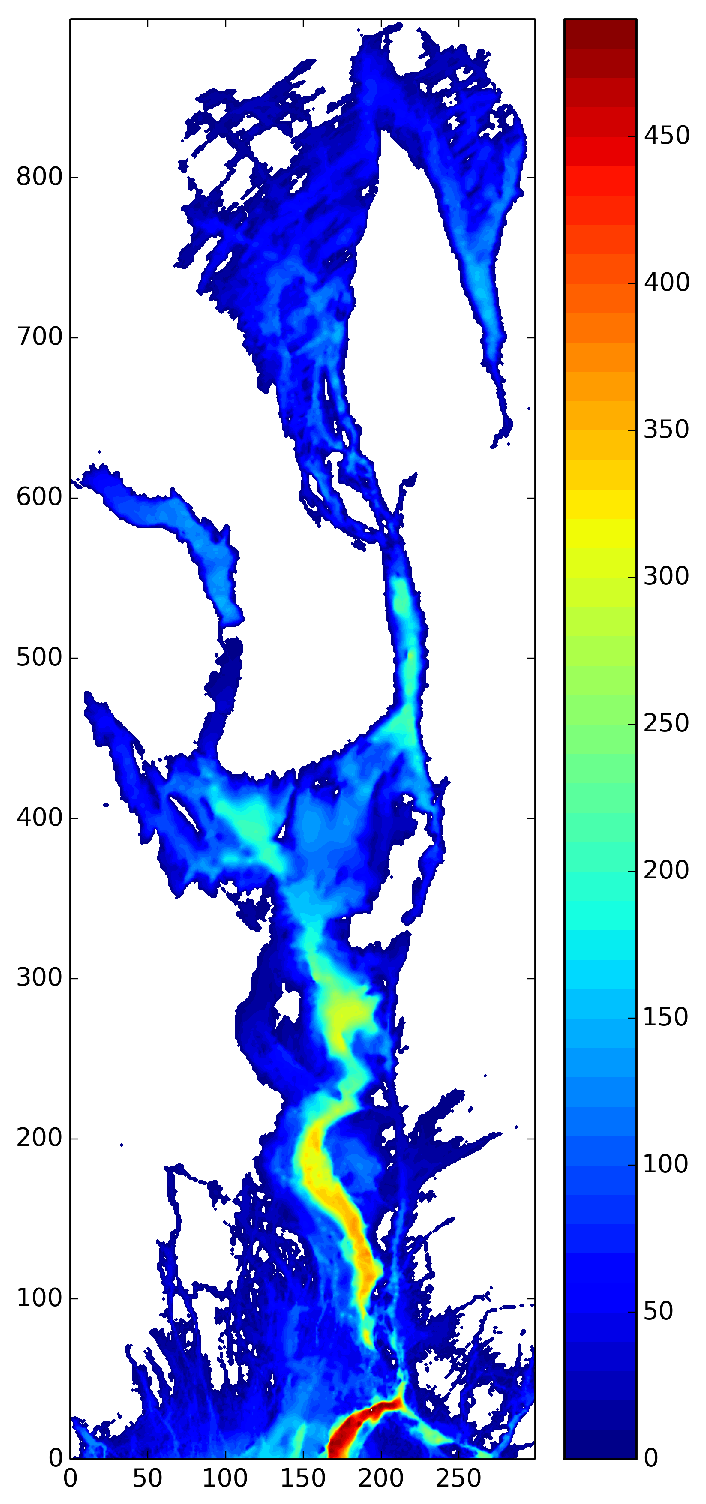
\includegraphics[height=8cm]{fjordos_cl}}
% Liggende
%   \rput[b]( 7.5,0.0){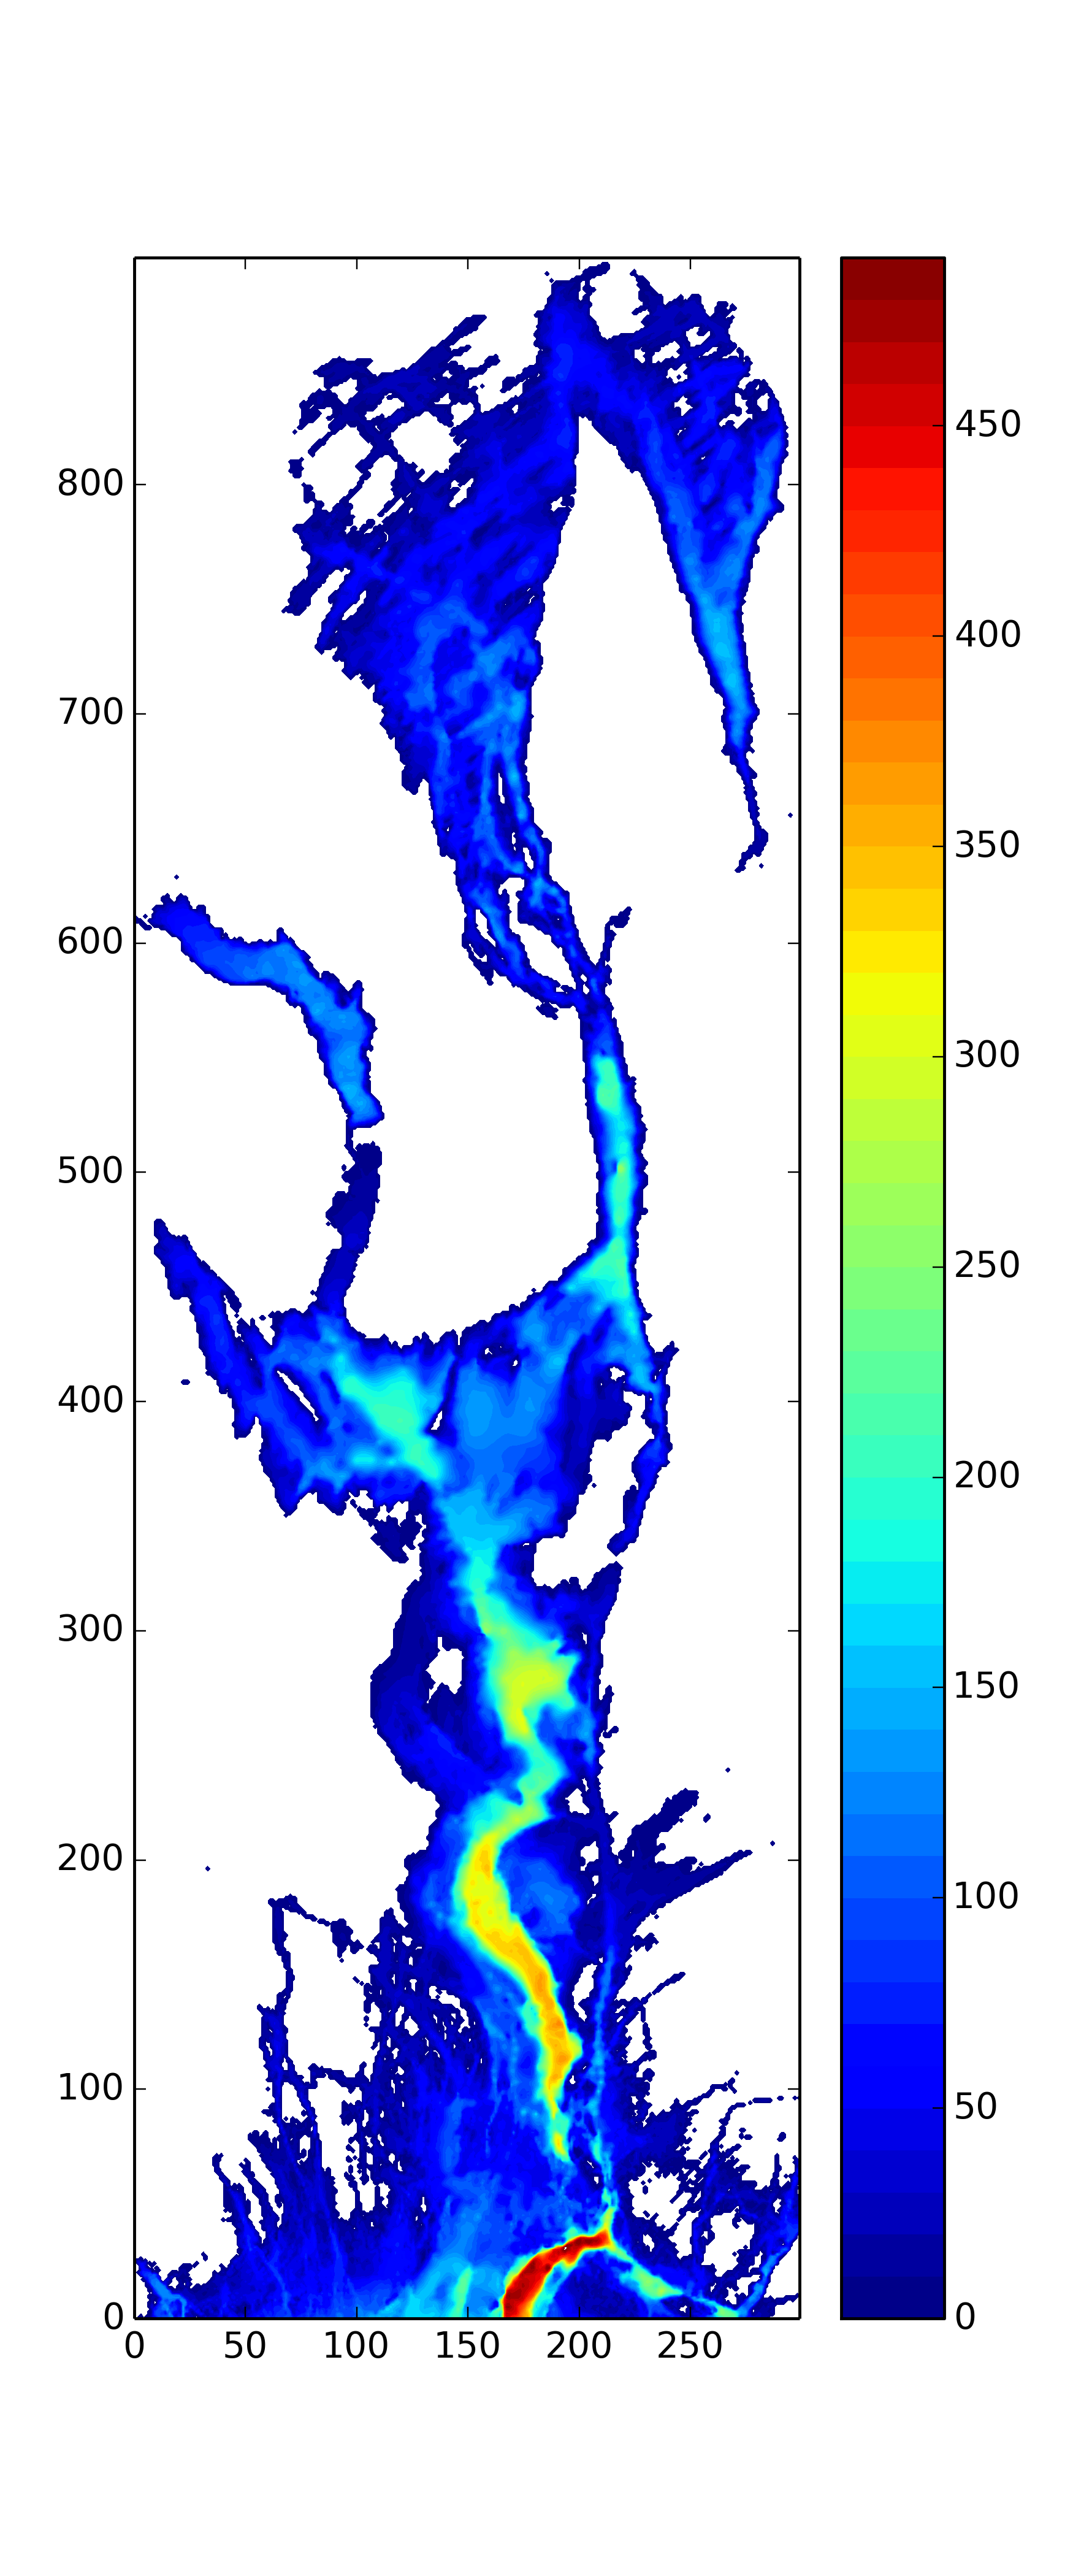
\includegraphics[angle=90,width=15.0cm,height=6.4865cm]{fjordos_roms}}
%   \rput[b]( 7.5,0.0){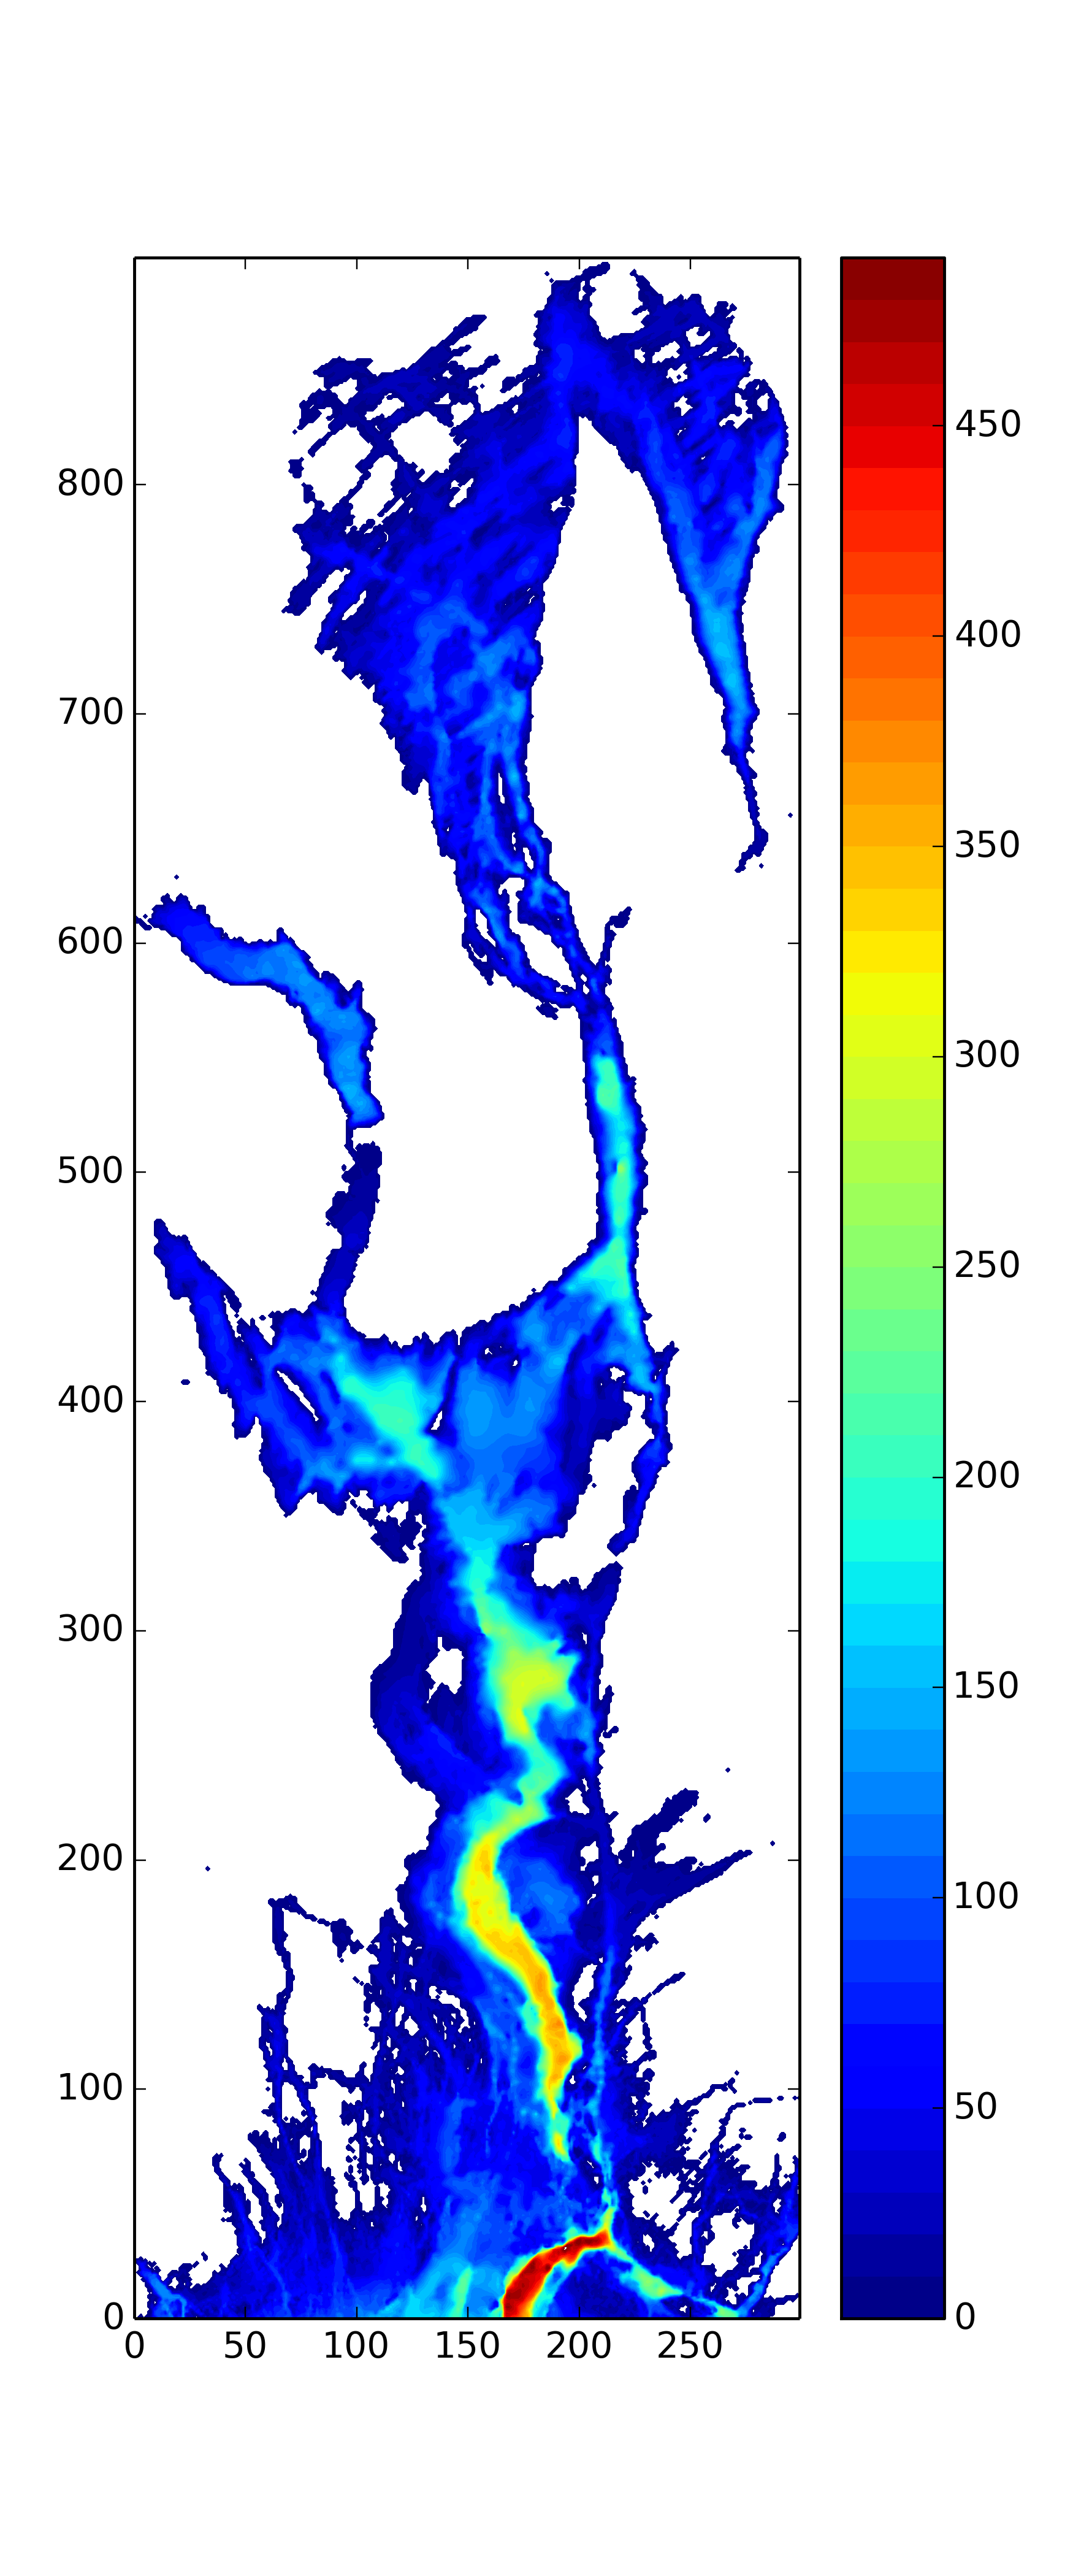
\includegraphics[height=8cm]{fjordos_roms}}
  \end{pspicture}
  \caption{\small The transformed curvilinear grid of the Oslofjord. The colors gives the depth in meters according to the color bar to the right. Model grid numbers associated with the curvilinear grid are given along the axes. There are 300 x 900 grid points.} 
  \label{fig:fjordos_cl}
 \end{center}
\end{figure}

